% !TEX root = micro_Lie_theory.tex

\section{序言}
\label{sec:intro}

在过去的几年里,机器人业界做出了巨大的努力来正确地用方程式确切表达估计问题。 
这是由于人们对方程解的精确性、一致性和稳定性的要求越来越高。 
事实上,对状态和测量、相关函数及其不确定性的适当建模对于实现这些目标至关重要。
这导致了涉及所谓“流形”的设计,在这种情况下,流形不亚于Lie群的光滑拓扑表面,这是状态表示的演化。
借助于Lie理论(Lie theory, LT),我们可以构造一个严格的微积分文献,精确而容易地处理不确定性、导数和积分。
通常,这些工作都集中在众所周知的旋转流形 $\SO(3)$ 和刚体运动 $\SE(3)$。

\begin{figure}[tb]
\centering
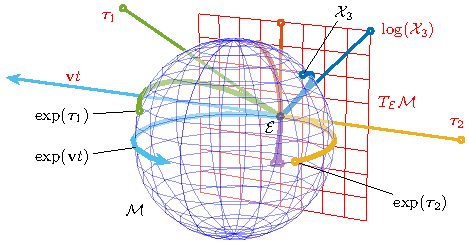
\includegraphics{figures/exponential}
\caption{Lie群与Lie代数关系的表示。
Lie代数 $\mtanat{\cM}{\cE}$ (红色平面)是Lie群流形 $\cM$ (这里用蓝色球面表示)在幺元 $\cE$ 处的切空间。
通过指数映射,每个通过Lie代数原点的直接路径 $\bfv t$ 产生一个围绕流形的路径 $\exp(\bfv t)$ ,流形沿着各自的测地线运行。 
相反的,群中的每个元素在李代数中都有一个等价项。
这种关系是如此深刻,以至于(几乎)群中的所有运算,那些曲线的和非线性的,在李代数中,这是一个线性向量空间,有一个精确的等价。
虽然 $\bbR^3$ 中的球面不是Lie群(我们只是把它当作一个可以画在纸上的表示),但 $\bbR^4$ 中的球面是Lie群,它描述了单位四元数群 --- 参见 \figRef{fig:manifold_q} 和 \exRef{ex:S3} 。
}
\label{fig:exponential}
\end{figure}

当第一次介绍Lie群时,从不同的角度看待它是很重要的。 
拓扑观点,参见 \figRef{fig:exponential} ,涉及流形的形状,并传达其与切空间和指数映射关系的强大直觉。
代数观点涉及群运算及其具体实现,允许利用代数性质来扩展闭式公式或简化它们。
几何视点在机器人学中特别有用,它将群元素与机体或参考坐标系中的位置、速度、方向和/或其它改变相关联。
原始坐标系可以用群的幺元来标识,并且流形上的任意其它点表示某个“局部”坐标系。
借助这些类比,Lie理论的许多数学抽象可以更接近向量空间、几何、运动学和其它更经典领域的直观概念。


Lie理论绝不简单。 
为了掌握Lie理论的最小概念,我们可以参考下面的三个参考文献。 
首先,Abbaspour的 \emph{``Basic Lie theory"}~\cite{ABBASPOUR-2007-Basic_Lie_theory} 有400多页。
也是类似的标题,Howe的 \emph{``Very basic Lie theory"}~\cite{Howe-Basic_Lie} 共有24(稠密的)页,有时被认为是必读的介绍。
最后,更现代、更著名的Stillwell的 \emph{``Naive Lie theory"}~\cite{STILLWELL-08} 共有200多页。
%
由于这些先例被标记为“基本的”、“非常基本的”和“幼稚的”,本文仅 \pageref{LastPage} 页的目的是进一步简化Lie理论 (因此标题中的形容词为 `微型(micro)')。
我们用两种方式来做。
首先,我们从Lie理论中选择一个素材的小子集。这个子集如此之小,以至于它仅仅是探索Lie理论的潜力。 
然而,它对于我们在机器人学中处理的估计问题(例如惯性预积分、里程计和SLAM、视觉伺服等)中的不确定性管理似乎非常有用,从而实现优化的优雅和严格的设计。
第二,我们用教学的方式来解释它,用大量的冗余来减少进入Lie理论的鸿沟,我们认为这仍然是必需的。
也就是说,我们坚持朝着这个方向努力,命名一个范例标题,Stillwell的文献 \cite{STILLWELL-08},并提供一个更简化的版本。
虽然我们试图将抽象级别保持在最低限度,但正文主体是通用的。
当应用到已知的群(旋转和运动矩阵、四元数等)时,插入的示例作为一般概念的基础。 
此外,许多标题非常冗长的插图再次解释了相同的概念。
我们特别关注Jacobian矩阵的计算 (这是一个在文献 \cite{STILLWELL-08} 中没有讨论的主题),它是大多数优化算法的关键,也是设计新算法时的麻烦源。
我们在最后一章给出了机器人定位和映射的应用实例,并在Lie理论基础上实现了EKF和非线性优化算法。
最后,几个附录包含了机器人学中最常用群最相关的详细信息:单位复数、四元数、二维和三维旋转矩阵、二维和三维刚体运动矩阵以及平凡平移群。


然而,我们对Lie理论最重要的简化是在范围方面。 
下面来自 
Howe~\cite{Howe-Basic_Lie} 的一段话可以帮助我们说明我们留下的东西:
%
``\emph{Lie理论的本质现象是人们可以用一种自然的方式联想到Lie群 $\cG$ 和它的Lie代数 $\frak{g}$。
Lie代数 $\frak{g}$ 首先是一个向量空间,其次被赋予一个称为Lie括号 [...] 的双线性非关联积。 
令人惊奇的是,群 $\cG$ 几乎完全由 $\frak{g}$ 和它的Lie括号决定。
因此,对于许多用途,可以用 $\frak{g}$ 代替 $\cG$。
因为 $\cG$ 是一个复杂的非线性对象,而 $\frak{g}$ 只是一个向量空间,所以使用 $\frak{g}$ 通常非常简单。
[...] 
这是Lie理论的力量源泉之一。%
}"
%
在文献 \cite{STILLWELL-08},Stillwell 甚至称为 ``\emph{Lie理论的奇迹}''.
在本次工作中,我们将有效地将Lie代数降级到第二平面,以支持它的等价向量空间 $\bbR^n$,因而根本不引入Lie括号。
因此,Lie群和它的Lie代数之间的联系在这里将不会像它应有的那样深刻。
我们的立场是,鉴于我们所预见的目标应用领域,这种(包含Lie括号的)素材通常是没有必要的。
%). 
此外,如果包含Lie括号在内,那么我们将无法达到清晰和有用的目标,因为读者将不得不进入数学概念,这些概念由于其抽象性或微妙性而变得不必要的复杂。



我们的努力与最近关于这个主题 ~\cite{BARFOOT-17-Estimation,EADE-Lie,forster2017-TRO} 的其它工作是一致的,这些工作也显示了带入Lie理论更进入机器人的需求。
我们的方法旨在让本文的目标读者,熟悉状态估计(Kalman滤波、基于图的优化等),但还不熟悉Lie理论的理论文献的读者,熟悉该理论。
%
为此,我们在符号方面采取了一些倡议,特别是在导数的定义方面,使其接近向量对应项,从而使链式规则清晰可见。
如前所述,我们实际上选择了避免Lie代数的素材,而是更喜欢研究它的同构切向量空间 $\bbR^n$,这是我们最终表示不确定性或(小)状态增量的地方。
所有这些步骤都是在绝对没有精度或准确性损失的情况下进行的,我们相信它们使得理解Lie理论及其工具的操作更容易。

本文伴随一个新的开源的只有头文件的 C++ 代码库,称为 \manif\ \cite{DERAY-20-manif},可以在这里找到: \url{https://github.com/artivis/manif} 。
\manif\ 实现广泛使用的群 $\SO(2)$, $\SO(3)$, $\SE(2)$ 和 $\SE(3)$,并支持创建分析 Jacobian 矩阵。
该库为易于使用、灵活性和性能而设计。

